

A commonly used validation experiment for multi-material models is that of a collapsing column of liquid, normally water, within an atmosphere or vacuum \citep{lakehal_interface_2002}, also known as the dam break problem.  In the experimental set-up a reservoir of water is held behind an impermeable barrier separating it from the rest of the tank.  The barrier is then quickly removed, allowing the water column to collapse and flood the remaining sections of the tank.  In the numerical analogue the initial condition is generally taken as the trapped water column, still behind the dam.  At the start of the simulation the barrier is imagined to have been removed instantaneously and switching on gravity, $|g| = 9.81$, causes the column to collapse.   Several experimental set-ups have been published and used as comparison and validation tools for numerical models \citep{martin_part_1952, greaves_simulation_2006}.  Those with water depth gauges distributed throughout the tank are particularly useful, allowing the direct comparison of data.  Furthermore, pressure gauges located on the tank walls or on any obstacles within the tank provide another useful validation tool.

\citet{zhou_nonlinear_1999} modelled a simple dam break problem experimentally in a $3.22\times2\times1m$ (length $\times$ height $\times$ depth) tank.  A reservoir of water $1.2\times0.6\times1m$ (length $\times$ height $\times$ depth) was held behind a barrier at one end of the tank.  Water depth gauges were placed at two points, marked H1 and H2 in Figure \ref{fig:zhouinitial}(a), at $x_1 = 2.725m$ and $2.228m$ respectively.  Additionally, a pressure gauge was located at the point marked P2 in Figure \ref{fig:zhouinitial}(a), at $x_2=0.16m$ on the wall facing the initial water column.

As no variations were introduced in the third dimension, the experiment is reproduced here numerically in two dimensions within the domain $\Omega$: $x_1 \in [0,3.22]$, $x_2 \in [0,2]$ \citep{lee_numerical_2002, colagrossi_numerical_2003, park_volume-of-fluid_2009}.  The initial condition of the water volume fraction is shown in Figure \ref{fig:zhouinitial}(a).  The presence of water is indicated as a grey region and the interface to air is delineated by contours at volume fraction values of $0.025$, $0.5$ and $0.975$.  The densities of the water and air are taken as $ 1,000kg\,m^{-2}$ and $1kg\,m^{-2}$ respectively.  Both fluids are treated inviscidly.  No information was given about the surface drag inside the tank during the experiment so instead, as the simulation is inviscid, free slip boundary conditions are imposed on the tank bottom, $x_2=0$, and sides, $x_1=0,\,3.22$.  The top of the tank, $x_2=2$, is left open.

\begin{figure}[tbp]
\hspace{1cm}(a)
\begin{center}
% modified from initial_setup.pdf_t, which was generated by xfig from initial_setup.fig
% modifications are a simple rescaling to 0.71 of original size
\begin{picture}(0,0)%
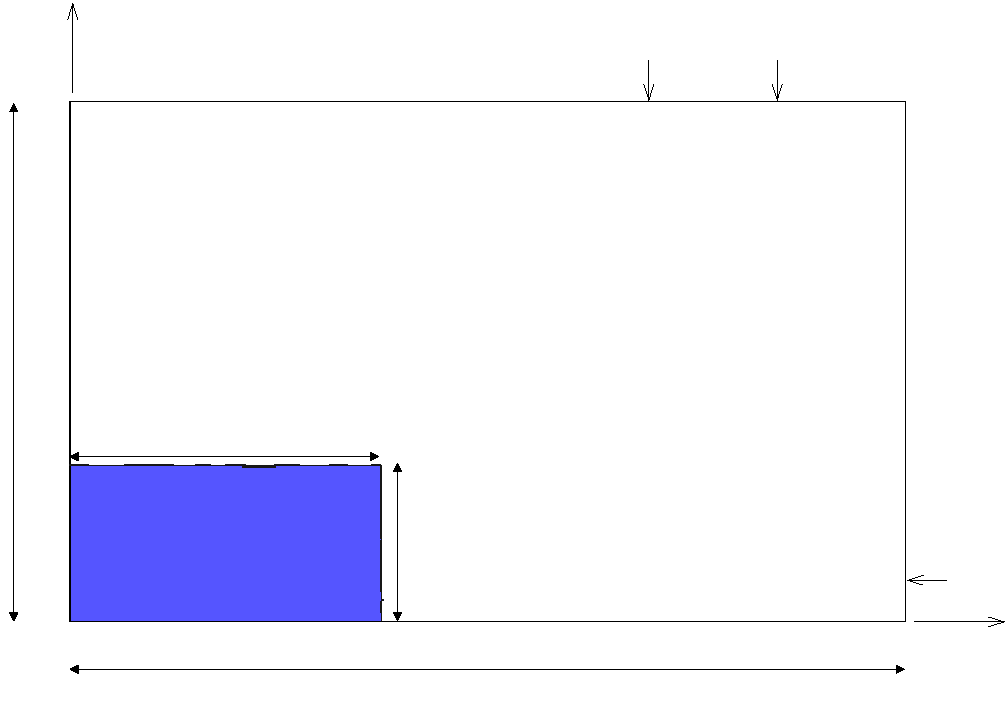
\includegraphics[scale=0.71]{examples_images/water_collapse/initial_setup.pdf}%
\end{picture}%
\setlength{\unitlength}{2942.24sp}%
%
\begingroup\makeatletter\ifx\SetFigFont\undefined%
\gdef\SetFigFont#1#2#3#4#5{%
  \reset@font\fontsize{#1}{#2pt}%
  \fontfamily{#3}\fontseries{#4}\fontshape{#5}%
  \selectfont}%
\fi\endgroup%
\begin{picture}(7677,5377)(2101,-9251)
\put(5761,-5326){\makebox(0,0)[lb]{\smash{{\SetFigFont{10}{12.0}{\familydefault}{\mddefault}{\updefault}{\color[rgb]{0,0,0}Air}%
}}}}
\put(2746,-4021){\makebox(0,0)[lb]{\smash{{\SetFigFont{10}{12.0}{\familydefault}{\mddefault}{\updefault}{\color[rgb]{0,0,0}$x_2$}%
}}}}
\put(5356,-4561){\makebox(0,0)[lb]{\smash{{\SetFigFont{10}{12.0}{\familydefault}{\mddefault}{\updefault}{\color[rgb]{0,0,0}$p = 0$}%
}}}}
\put(7111,-4246){\makebox(0,0)[b]{\smash{{\SetFigFont{10}{12.0}{\familydefault}{\mddefault}{\updefault}{\color[rgb]{0,0,0}2.228$m$}%
}}}}
\put(8101,-4246){\makebox(0,0)[b]{\smash{{\SetFigFont{10}{12.0}{\familydefault}{\mddefault}{\updefault}{\color[rgb]{0,0,0}2.725$m$}%
}}}}
\put(7066,-4021){\makebox(0,0)[b]{\smash{{\SetFigFont{10}{12.0}{\familydefault}{\mddefault}{\updefault}{\color[rgb]{0,0,0}H2}%
}}}}
\put(8056,-4021){\makebox(0,0)[b]{\smash{{\SetFigFont{10}{12.0}{\familydefault}{\mddefault}{\updefault}{\color[rgb]{0,0,0}H1}%
}}}}
\put(9586,-8881){\makebox(0,0)[lb]{\smash{{\SetFigFont{10}{12.0}{\familydefault}{\mddefault}{\updefault}{\color[rgb]{0,0,0}$x_1$}%
}}}}
\put(9676,-8341){\makebox(0,0)[b]{\smash{{\SetFigFont{10}{12.0}{\familydefault}{\mddefault}{\updefault}{\color[rgb]{0,0,0}0.16$m$}%
}}}}
\put(9676,-8116){\makebox(0,0)[b]{\smash{{\SetFigFont{10}{12.0}{\familydefault}{\mddefault}{\updefault}{\color[rgb]{0,0,0}P2}%
}}}}
\put(5761,-9196){\makebox(0,0)[b]{\smash{{\SetFigFont{10}{12.0}{\familydefault}{\mddefault}{\updefault}{\color[rgb]{0,0,0}3.22$m$}%
}}}}
\put(2116,-6631){\makebox(0,0)[rb]{\smash{{\SetFigFont{10}{12.0}{\familydefault}{\mddefault}{\updefault}{\color[rgb]{0,0,0}2.0$m$}%
}}}}
\put(4051,-7261){\makebox(0,0)[rb]{\smash{{\SetFigFont{10}{12.0}{\familydefault}{\mddefault}{\updefault}{\color[rgb]{0,0,0}1.2$m$}%
}}}}
\put(5446,-8071){\makebox(0,0)[b]{\smash{{\SetFigFont{10}{12.0}{\familydefault}{\mddefault}{\updefault}{\color[rgb]{0,0,0}0.6$m$}%
}}}}
\put(3601,-7036){\makebox(0,0)[lb]{\smash{{\SetFigFont{10}{12.0}{\familydefault}{\mddefault}{\updefault}{\color[rgb]{0,0,0}Water}%
}}}}
\put(5896,-8836){\makebox(0,0)[b]{\smash{{\SetFigFont{10}{12.0}{\familydefault}{\mddefault}{\updefault}{\color[rgb]{0,0,0}$u_in_i = 0$}%
}}}}
\put(2476,-6586){\rotatebox{90.0}{\makebox(0,0)[b]{\smash{{\SetFigFont{10}{12.0}{\familydefault}{\mddefault}{\updefault}{\color[rgb]{0,0,0}$u_in_i = 0$}%
}}}}}
\put(9136,-6586){\rotatebox{270.0}{\makebox(0,0)[b]{\smash{{\SetFigFont{10}{12.0}{\familydefault}{\mddefault}{\updefault}{\color[rgb]{0,0,0}$u_in_i = 0$}%
}}}}}
\end{picture}%

\end{center}
\hspace{1cm}(b)
\begin{center}
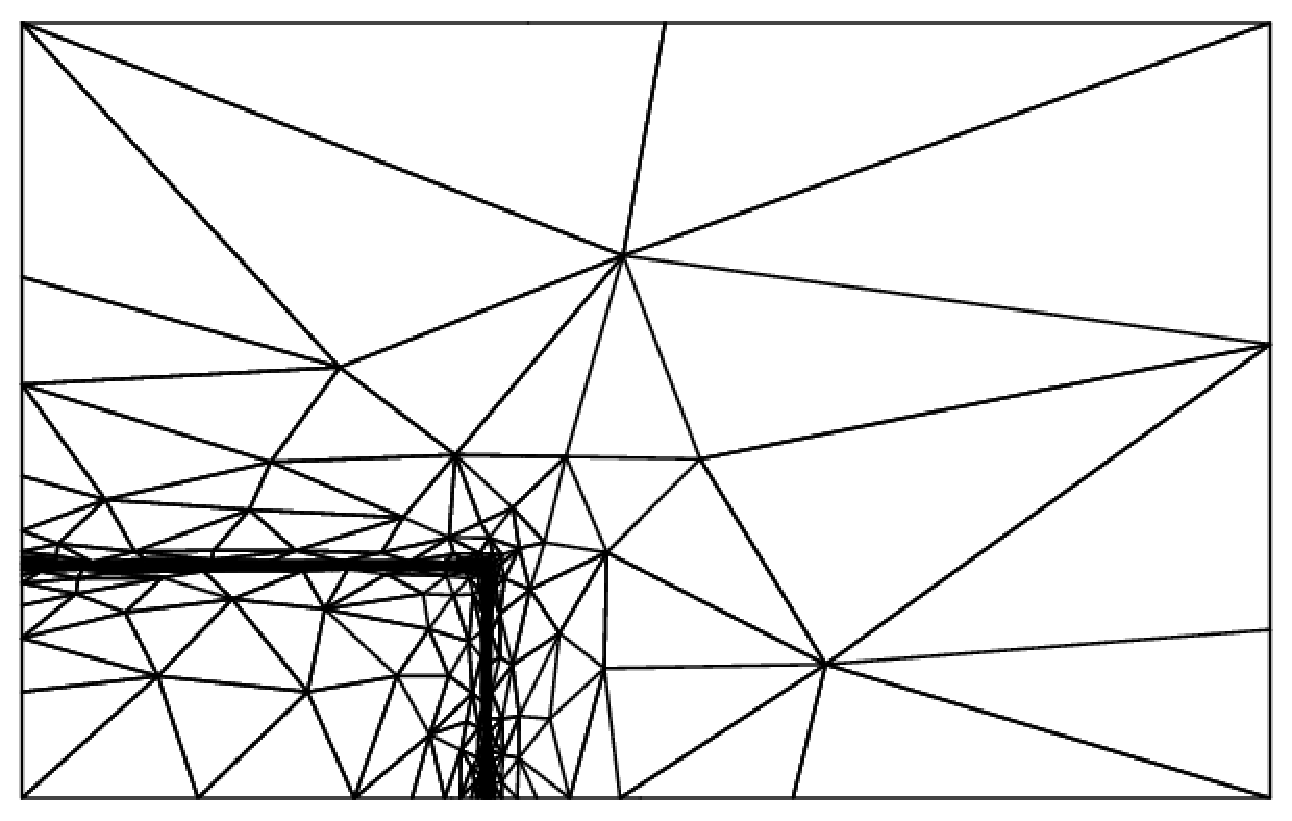
\includegraphics[width=10.2cm, trim=2.5cm 4.5cm 2.5cm 4.5cm, clip=true]{pictures/water_collapse_0_mesh.pdf}
\end{center}
\caption{(a) Initial set-up of the water volume fraction, $\alpha^1$, and the velocity and pressure boundary conditions for the two-dimensional water column collapse validation problem \citep{zhou_nonlinear_1999}. The presence of water is indicated as a grey region and the interface to air is delineated by contours of the volume fraction at $0.025$, $0.5$ and $0.975$.  The locations of the pressure (P2) and water depth gauges (H1, H2) are also indicated. (b) The adapted mesh used to represent the initial conditions.}
\label{fig:zhouinitial}
\end{figure}

\begin{figure}[tbp]
\begin{center}
% \newcolumntype{V}{>{\centering\arraybackslash} m{7cm} }
\begin{tabular}{ll}
\hspace{2cm}(i) Fixed Mesh  & \hspace{1.8cm}(ii) Adaptive Mesh\\
(a) $t = 0.5$ \\
\includegraphics[width=7cm, trim=2.5cm 4.5cm 2.5cm 4.5cm, clip=true]{pictures/zhou/water_collapse_100_fixed.png} & 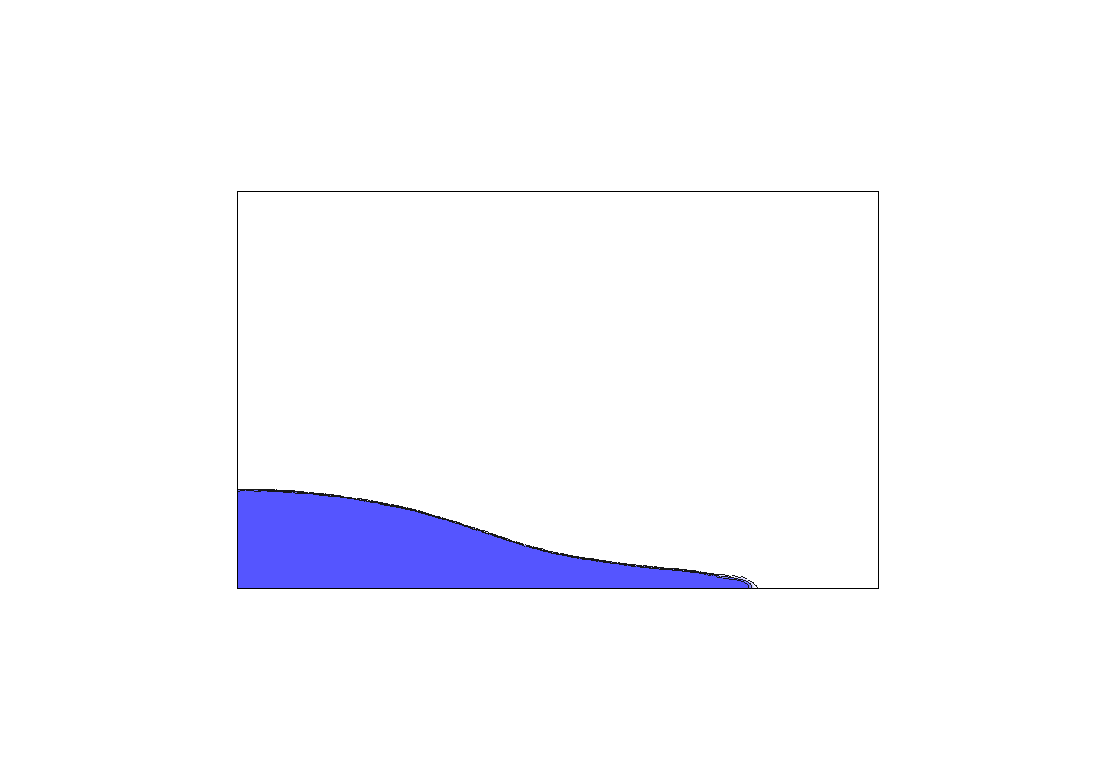
\includegraphics[width=7cm, trim=2.5cm 4.5cm 2.5cm 4.5cm, clip=true]{pictures/zhou/water_collapse_100.png} \\
(b) $t = 1.0$ \\
\includegraphics[width=7cm, trim=2.5cm 4.5cm 2.5cm 4.5cm, clip=true]{pictures/zhou/water_collapse_200_fixed.png} & 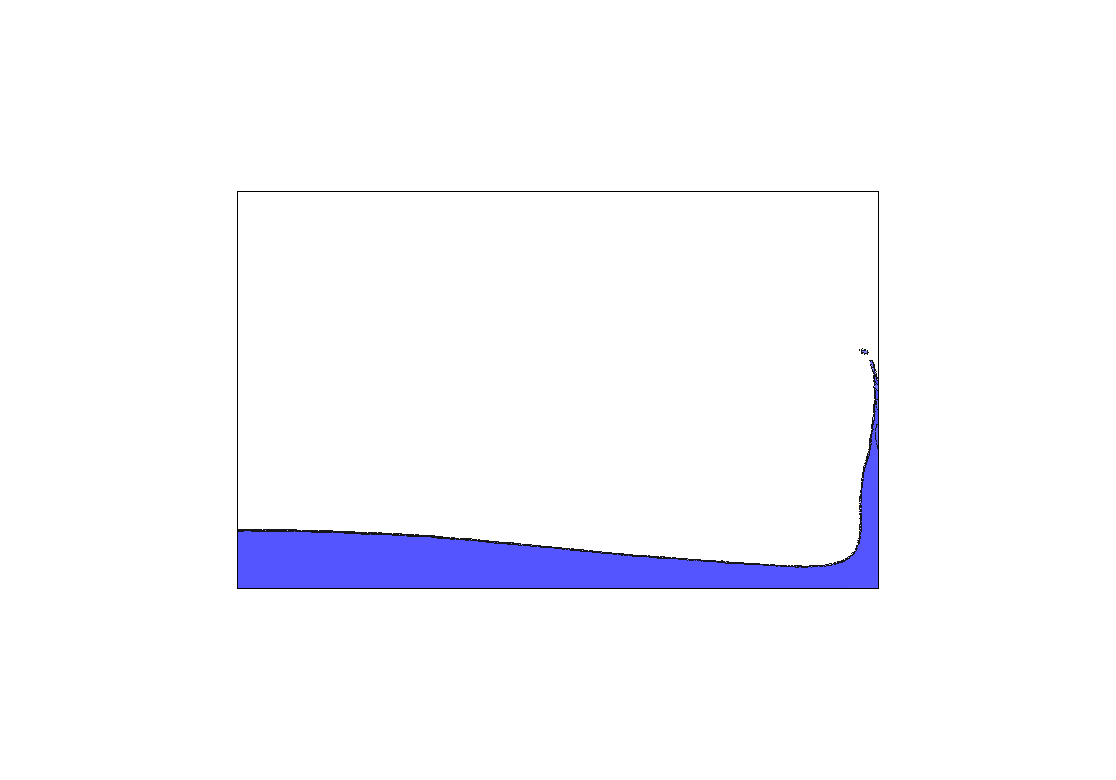
\includegraphics[width=7cm, trim=2.5cm 4.5cm 2.5cm 4.5cm, clip=true]{pictures/zhou/water_collapse_200.png} \\
(c) $t = 1.5$ \\
\includegraphics[width=7cm, trim=2.5cm 4.5cm 2.5cm 4.5cm, clip=true]{pictures/zhou/water_collapse_300_fixed.png} & 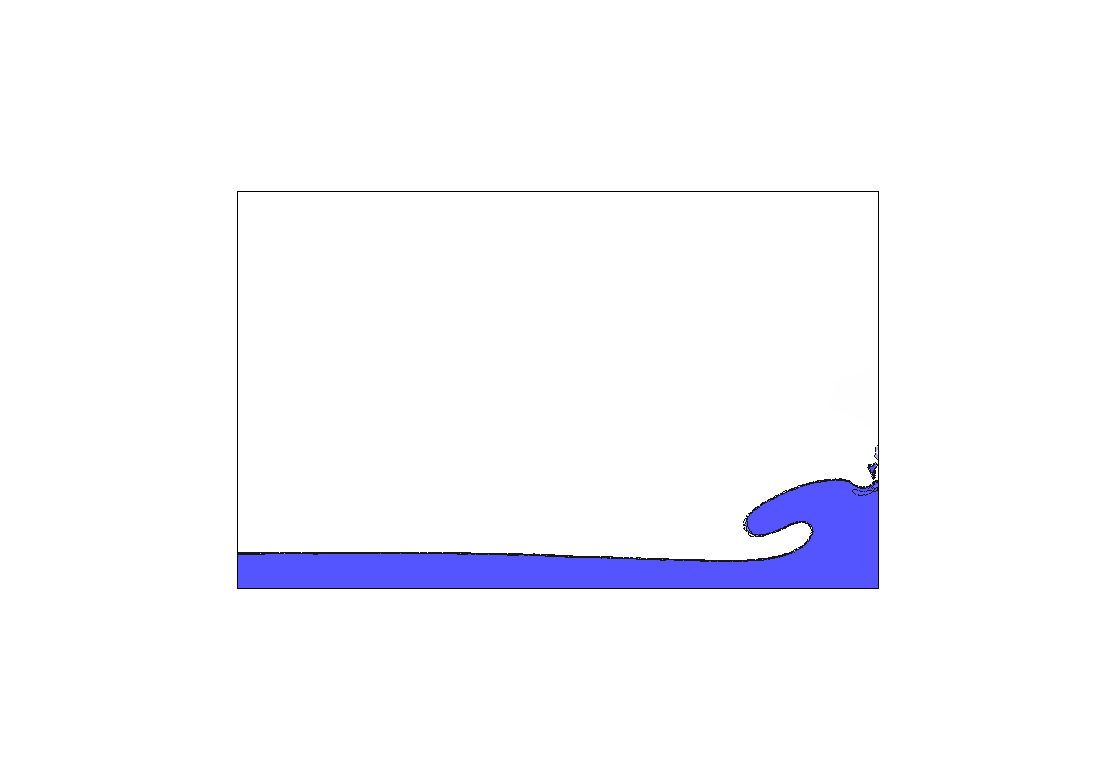
\includegraphics[width=7cm, trim=2.5cm 4.5cm 2.5cm 4.5cm, clip=true]{pictures/zhou/water_collapse_300.png} \\
(d) $t = 1.625$ \\
\includegraphics[width=7cm, trim=2.5cm 4.5cm 2.5cm 4.5cm, clip=true]{pictures/zhou/water_collapse_325_fixed.png} & \includegraphics[width=7cm, trim=2.5cm 4.5cm 2.5cm 4.5cm, clip=true]{pictures/zhou/water_collapse_325.png} \\
\end{tabular}
\caption{The evolution of the water volume fraction, $\alpha^1$, over several timesteps on a fixed $238\times158$ mesh (i) and an adaptive mesh with the same minimum edge length (ii).  The presence of water, $\alpha^1=1$, is indicated as a grey region and the interface to air, $\alpha^1=0$, is delineated by contours at $\alpha^1 = 0.025$, $0.5$ and $0.975$.}
\end{center}
\end{figure}

The water volume fraction, $\alpha^1$, is advected using HyperC on the control volume mesh dual to the piecewise linear finite element parent mesh while the velocity and pressure are discretised using the P0P1$_{\text{CV}}$ element pair with $\theta=1/2$ and $\theta_i=1/2$.  The domain is initially discretised using the same resolution as the medium case of \citet{park_volume-of-fluid_2009}, with $238\times158$ grid points distributed evenly throughout the domain except in a high resolution zone within $0.1m$ of the lower and right boundaries where $43$ points are concentrated.  The timestep is selected to achieve a Courant number of $2.5$ while the advection equation uses approximately $10$ subcycles so the volume fraction is advected at a Courant number of $0.25$.  Several timesteps of this simulation can be seen in Figure \ref{fig:zhouwholea}(i) where the interface is represented by contours of the water volume fraction, $\alpha^1$, at $0.025$, $0.5$ and $0.975$.

\addtocounter{figure}{-1}
\begin{figure}[tbp]
\begin{center}
% \newcolumntype{V}{>{\centering\arraybackslash} m{7cm} }
\begin{tabular}{ll}
\hspace{2cm}(i) Fixed Mesh  & \hspace{1.8cm}(ii) Adaptive Mesh\\
(e) $t = 1.75$ \\
\includegraphics[width=7cm, trim=2.5cm 4.5cm 2.5cm 4.5cm, clip=true]{pictures/zhou/water_collapse_350_fixed.png} & 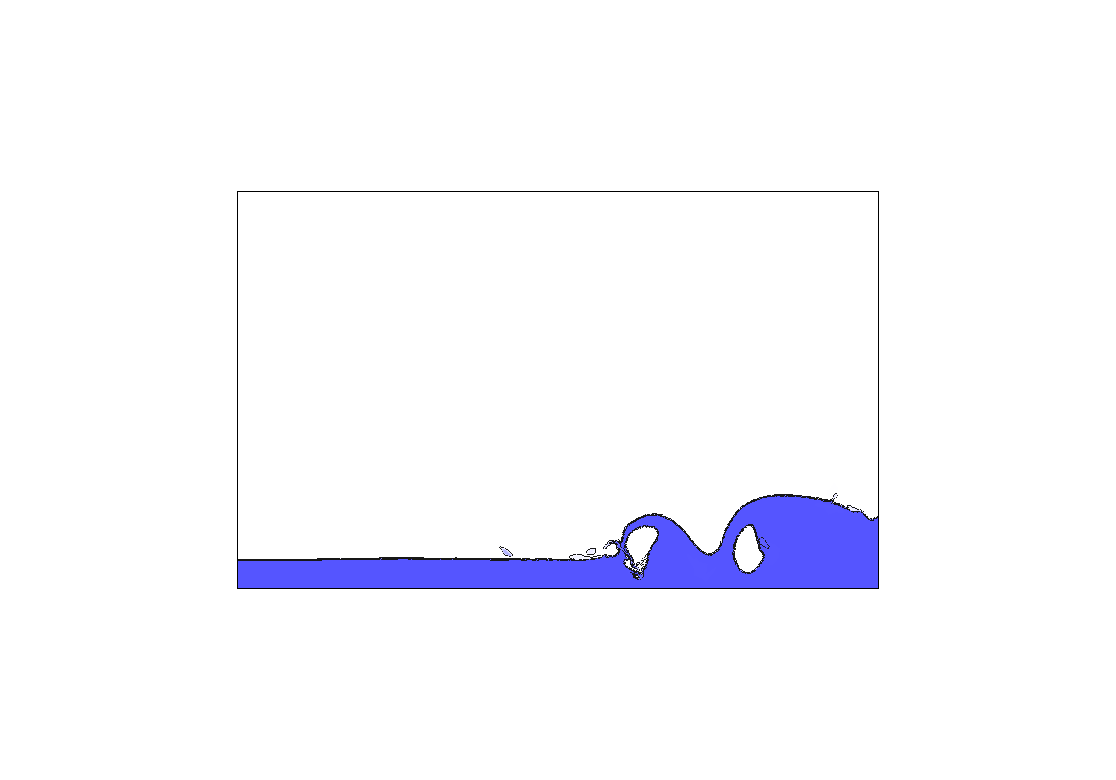
\includegraphics[width=7cm, trim=2.5cm 4.5cm 2.5cm 4.5cm, clip=true]{pictures/zhou/water_collapse_350.png} \\
(f) $t = 1.875$ \\
\includegraphics[width=7cm, trim=2.5cm 4.5cm 2.5cm 4.5cm, clip=true]{pictures/zhou/water_collapse_375_fixed.png} & \includegraphics[width=7cm, trim=2.5cm 4.5cm 2.5cm 4.5cm, clip=true]{pictures/zhou/water_collapse_375.png} \\
(g) $t = 2.0$ \\
\includegraphics[width=7cm, trim=2.5cm 4.5cm 2.5cm 4.5cm, clip=true]{pictures/zhou/water_collapse_400_fixed.png} & 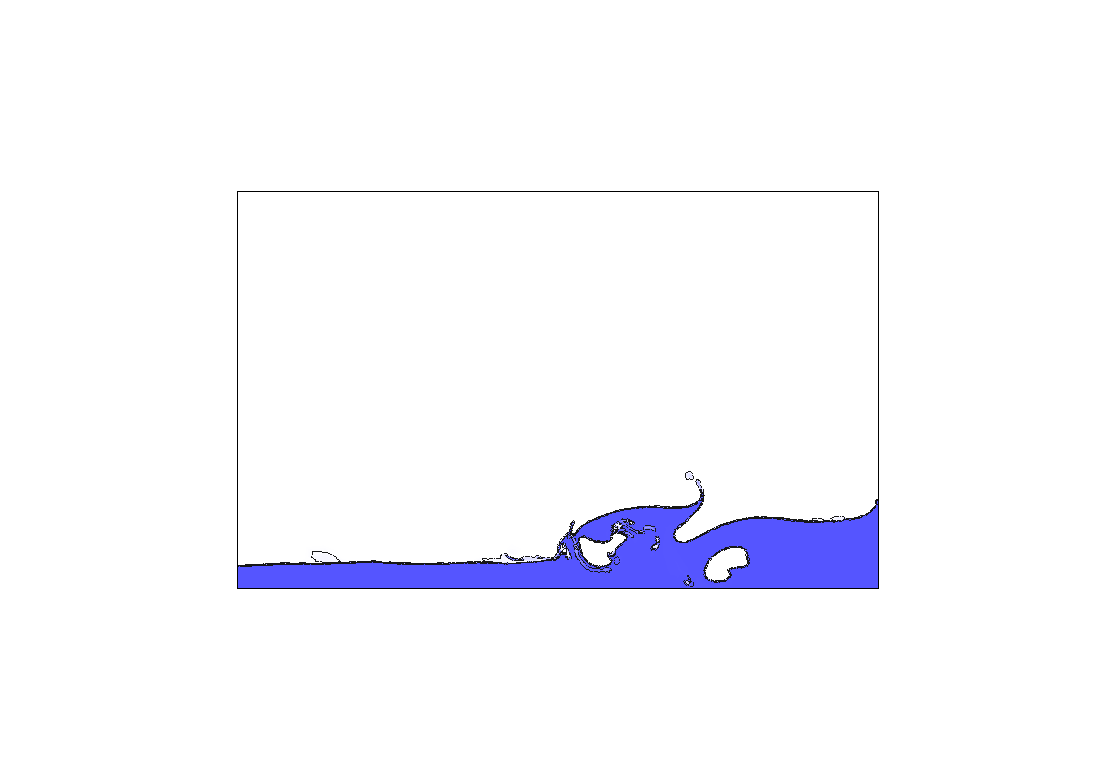
\includegraphics[width=7cm, trim=2.5cm 4.5cm 2.5cm 4.5cm, clip=true]{pictures/zhou/water_collapse_400.png} \\
(h) $t = 2.5$ \\
\includegraphics[width=7cm, trim=2.5cm 4.5cm 2.5cm 4.5cm, clip=true]{pictures/zhou/water_collapse_500_fixed.png} & 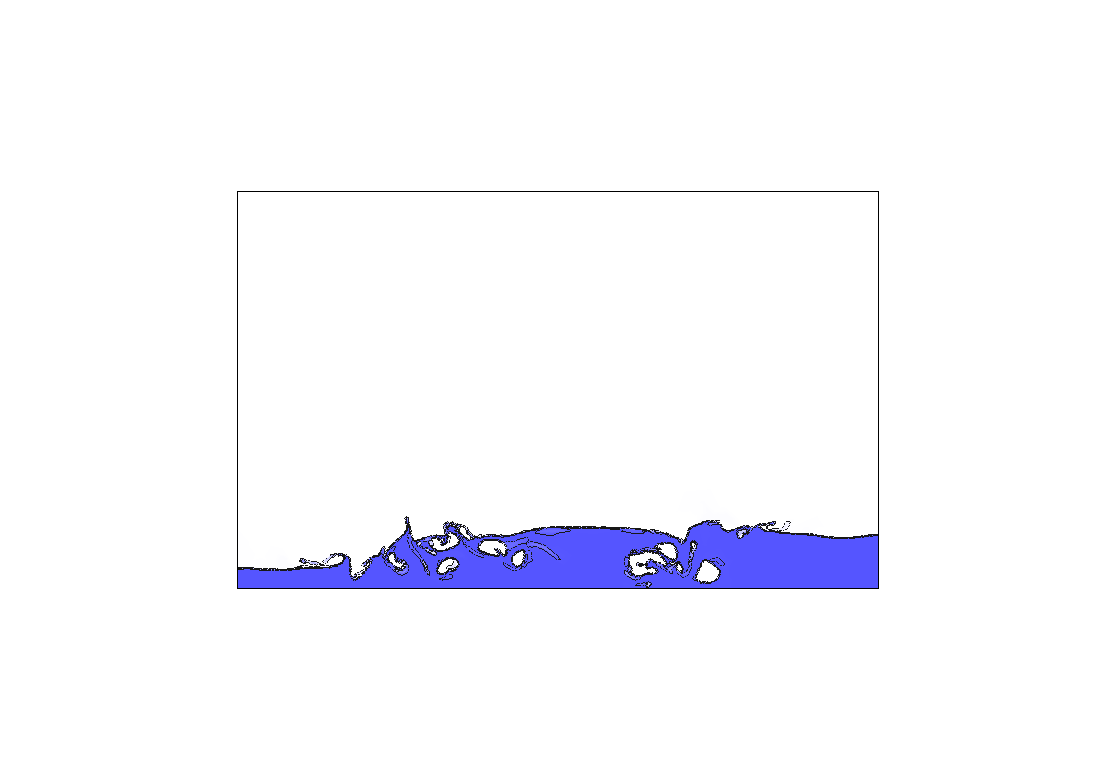
\includegraphics[width=7cm, trim=2.5cm 4.5cm 2.5cm 4.5cm, clip=true]{pictures/zhou/water_collapse_500.png} \\
\end{tabular}
\caption{\emph{cont.} The evolution of the water volume fraction, $\alpha^1$, over several timesteps on a fixed $238\times158$ mesh (i) and an adaptive mesh with the same minimum edge length (ii).  The presence of water, $\alpha^1=1$, is indicated as a grey region and the interface to air, $\alpha^1=0$, is delineated by contours at $\alpha^1 = 0.025$, $0.5$ and $0.975$.}
\label{fig:zhouwholea}
\end{center}
\end{figure}

Therefore an adaptive simulation was also performed with the minimum edge length constrained to $2mm$, equivalent to the high resolution zone in the fixed mesh simulation.  The upper bound on the edge lengths was specified as half the domain length and height in each dimension.  The pressure and water volume fraction were directly adapted to using interpolation error bounds, $\hat{\epsilon}$, of $1,000$ and $0.05$ respectively.  As the velocity is element centred it was first projected to the vertices before being adapted to with an interpolation error bound of $1$ for each component.  Given the ranges of these fields seen in the fixed mesh runs these correspond to desired errors of less than 5\% for each field.  As in Section \ref{sec:adaptmesh} the volume fraction is transferred between successive meshes using a minimally diffusive bounded projection algorithm.  The velocity is transferred using a straightforward projection while the pressure is consistently interpolated using the linear basis functions from its parent mesh.  All the remaining adaptivity settings are the same as used in Figure \ref{fig:shearadaptgood} with metric advection, edge length gradation and the solenoidal projection of the velocity interpolant following mesh optimisation.  The initial mesh using these settings is shown in Figure \ref{fig:zhouinitial}(b).

\begin{figure}[tbp]
\begin{center}
% \newcolumntype{V}{>{\centering\arraybackslash} m{7cm} }
\begin{tabular}{ll}
(a) $t = 0.5$ & (b) $t = 1.0$\\
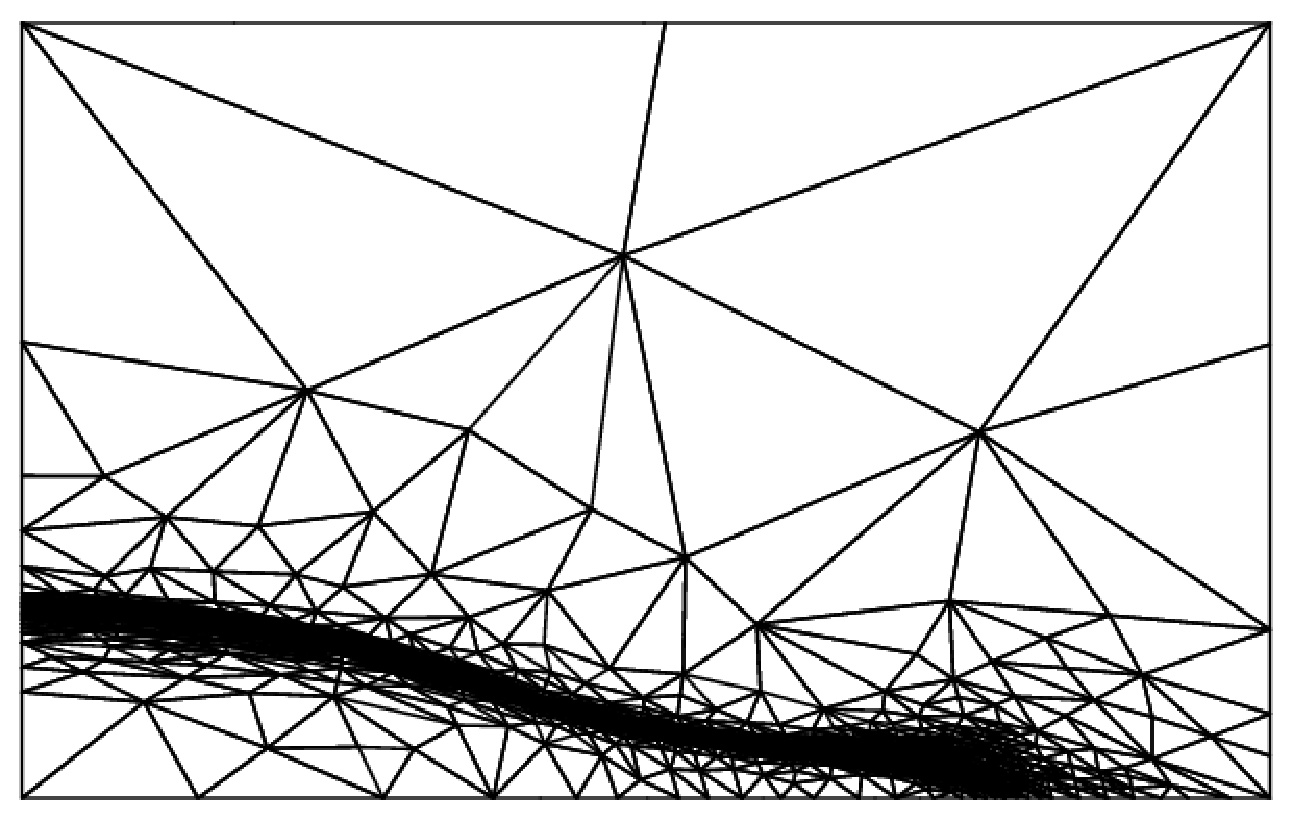
\includegraphics[width=7cm, trim=2.5cm 4.5cm 2.5cm 4.5cm, clip=true]{pictures/zhou/water_collapse_100_mesh.pdf} & 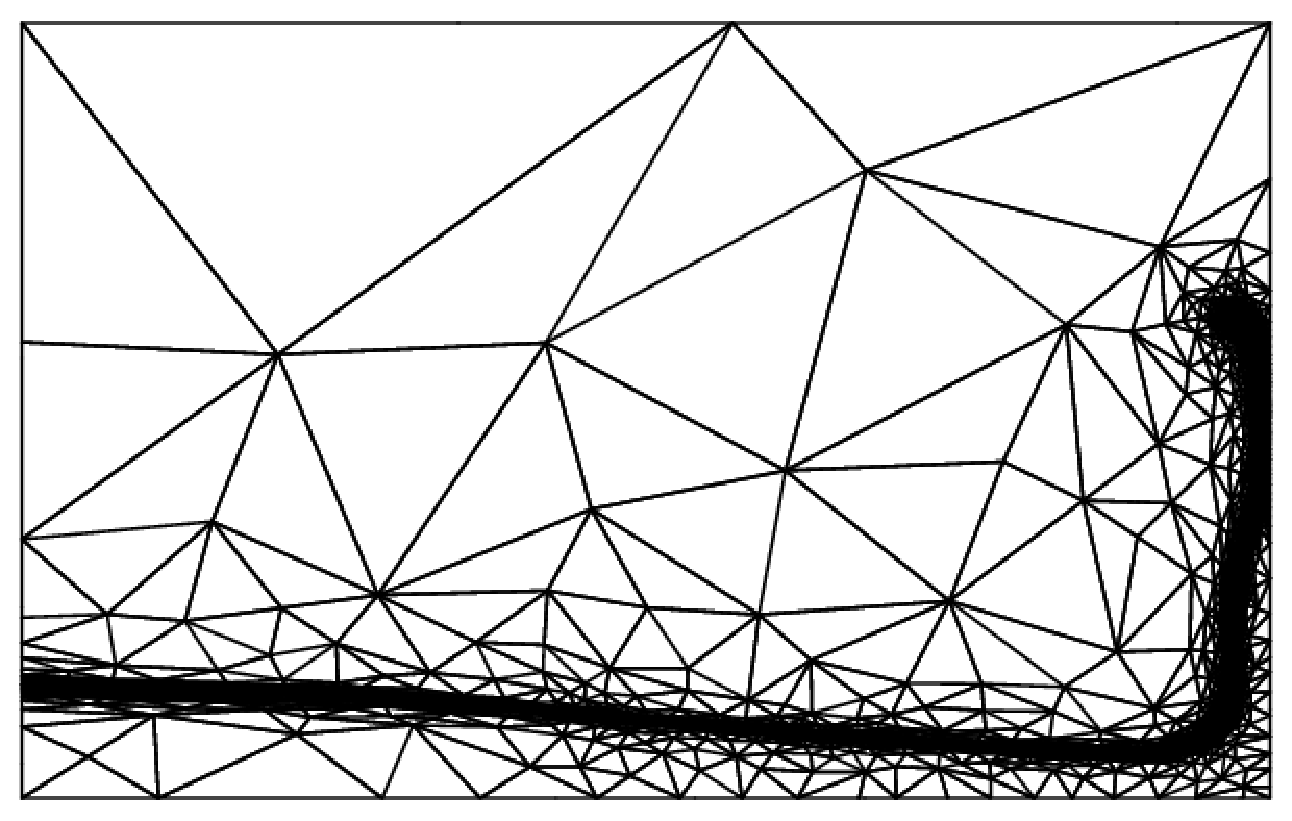
\includegraphics[width=7cm, trim=2.5cm 4.5cm 2.5cm 4.5cm, clip=true]{pictures/zhou/water_collapse_200_mesh.pdf} \\
(c) $t = 1.5$ & (d) $t = 1.625$ \\
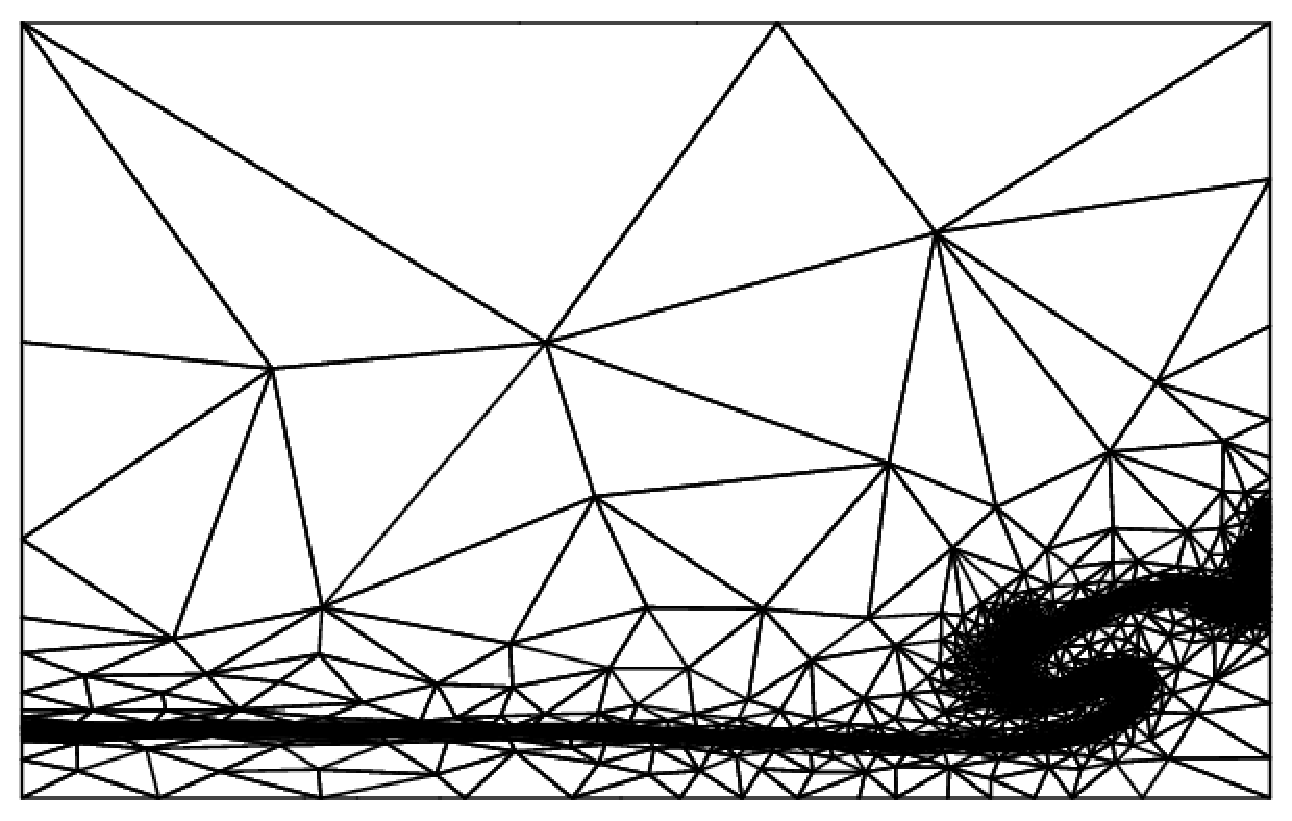
\includegraphics[width=7cm, trim=2.5cm 4.5cm 2.5cm 4.5cm, clip=true]{pictures/zhou/water_collapse_300_mesh.pdf} & \includegraphics[width=7cm, trim=2.5cm 4.5cm 2.5cm 4.5cm, clip=true]{pictures/zhou/water_collapse_325_mesh.pdf} \\
(e) $t = 1.75$ & (f) $t = 1.875$ \\
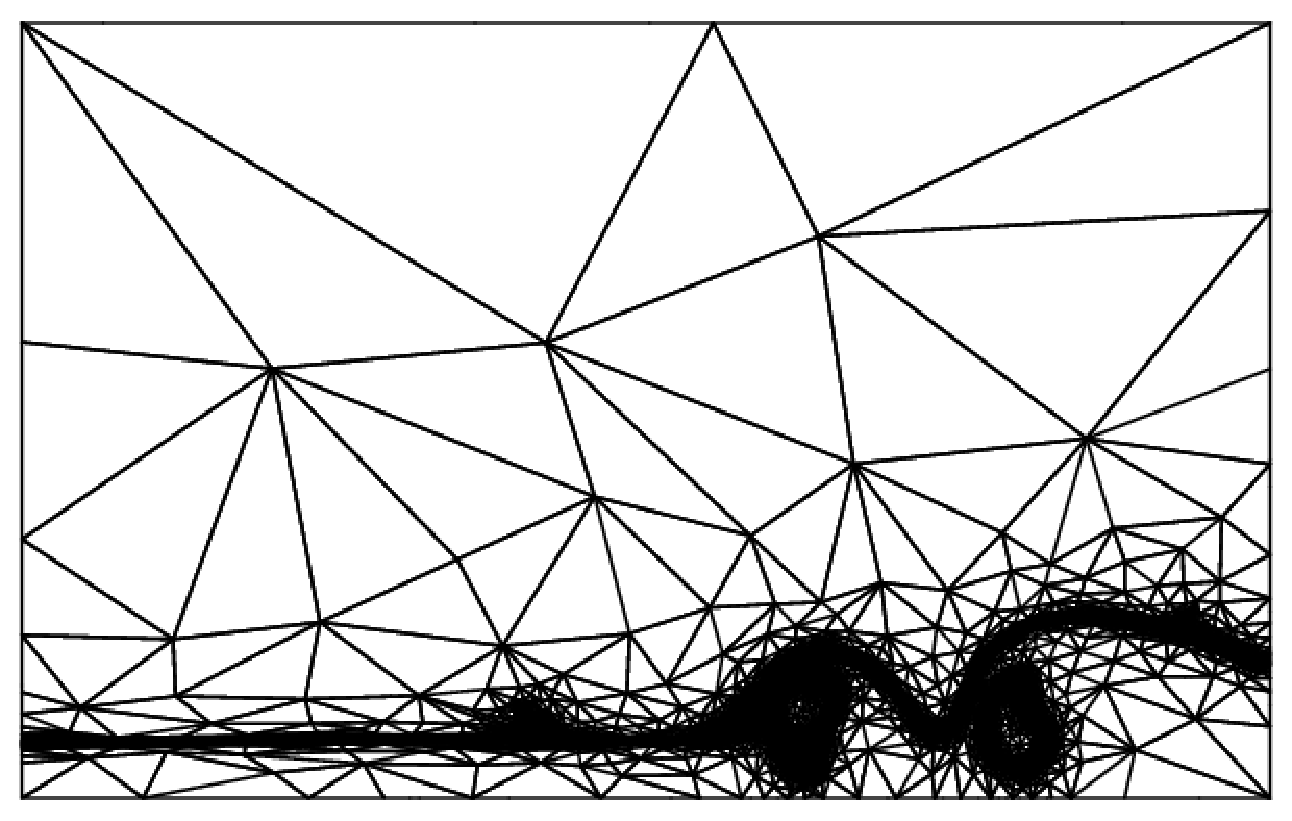
\includegraphics[width=7cm, trim=2.5cm 4.5cm 2.5cm 4.5cm, clip=true]{pictures/zhou/water_collapse_350_mesh.pdf} & \includegraphics[width=7cm, trim=2.5cm 4.5cm 2.5cm 4.5cm, clip=true]{pictures/zhou/water_collapse_375_mesh.pdf} \\
(g) $t = 2.0$ & (h) $t = 2.5$ \\
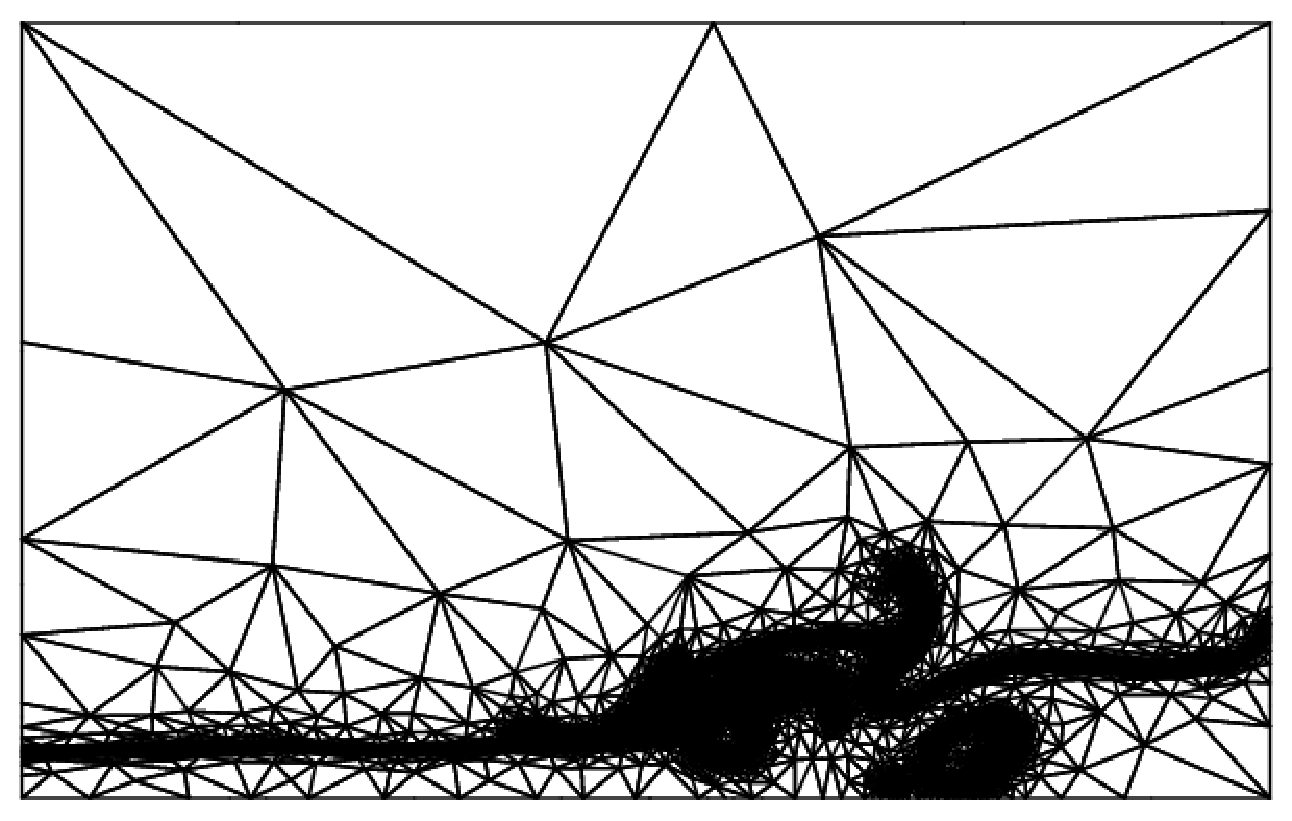
\includegraphics[width=7cm, trim=2.5cm 4.5cm 2.5cm 4.5cm, clip=true]{pictures/zhou/water_collapse_400_mesh.pdf} & 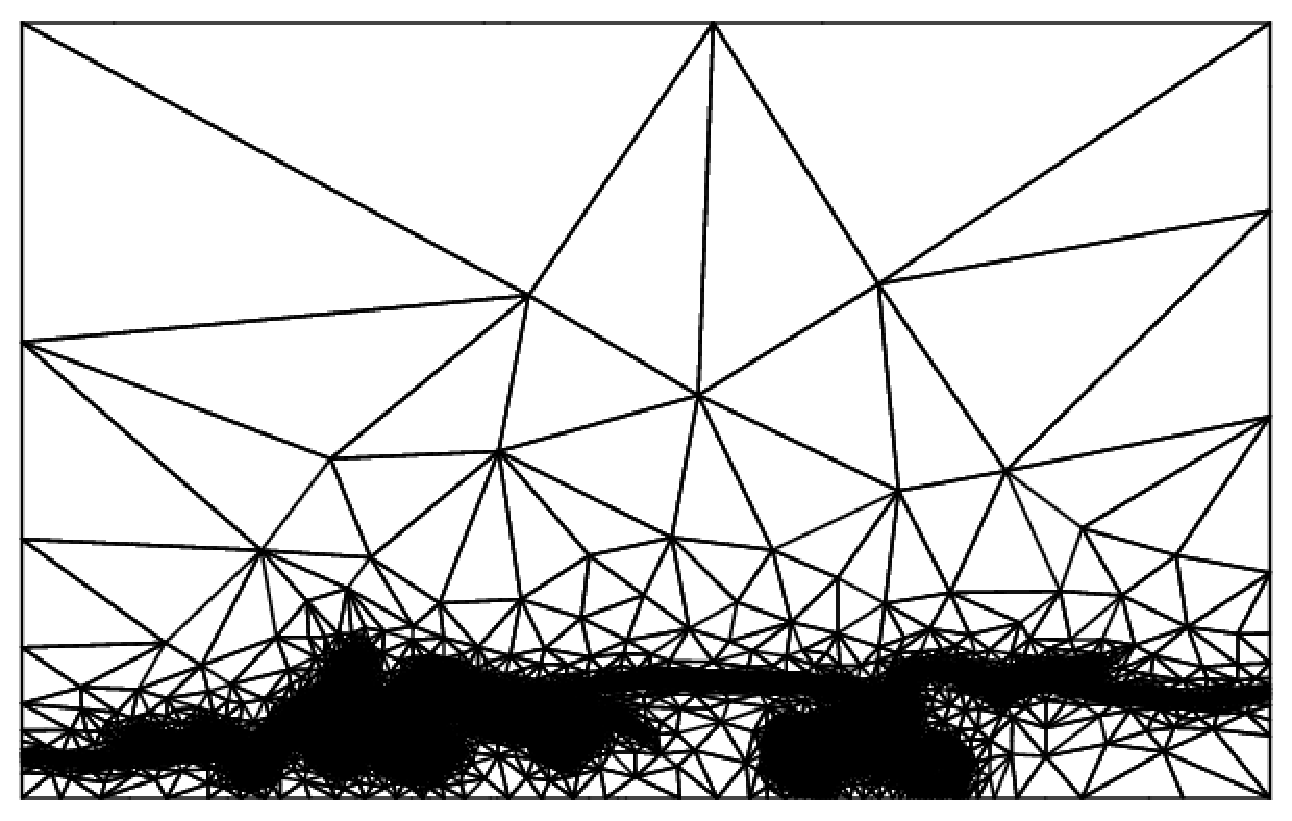
\includegraphics[width=7cm, trim=2.5cm 4.5cm 2.5cm 4.5cm, clip=true]{pictures/zhou/water_collapse_500_mesh.pdf} \\
\end{tabular}
\caption{The evolution of the adaptive mesh over the same timesteps displayed in Figure \ref{fig:zhouwholea}(ii).  The mesh can be seen to closely follow the interface between the water and air.}
\label{fig:zhouwholemesh}
\end{center}
\end{figure}

Results using the adaptive mesh are presented alongside the fixed mesh results in Figure \ref{fig:zhouwholea}(ii) while the corresponding adapted meshes are shown in Figure \ref{fig:zhouwholemesh}.  The two sets of results are very similar showing the column collapse (Figure \ref{fig:zhouwholea}(a)), run-up against the opposing wall (Figure \ref{fig:zhouwholea}(b)) and subsequent overturning wave (Figure \ref{fig:zhouwholea}(c, d)) and entrainment of air bubbles (Figure \ref{fig:zhouwholea}(e--h)).  However, discrepancies between the solutions do occur.  The adaptive mesh displays closely packed contours along the entire length of the interface throughout the simulation, not just towards the base in the early timesteps as in the fixed mesh run.  Furthermore, very few mixed cells are visible in the adaptive mesh run, even towards the end when the dynamics become increasingly complicated.  This is a consequence of finer resolution around the entire interface throughout the adaptive mesh simulation.

While the broad dynamics are similar between the two simulations the adaptive mesh run is seen to have a lower wave run-up on the opposing wall (Figure \ref{fig:zhouwholea}(b)), resulting in a slightly different overturning wave (Figure \ref{fig:zhouwholea}(c)).  It is unclear if this is a result of having less mixing in the interface zone, resulting in a better defined, less buoyant water region, or whether some interaction between the adapting mesh and the advection is taking place, as was seen in Figure \ref{fig:shearadaptbad}.  Wave run-up using adapting meshes is investigated further in Chapter \ref{chap:multimat}.  After about $t=1.5s$ the overturning wave impacts with the basal water layer.  At this point the dynamics become increasingly complex and discrepancies between the adaptive and fixed mesh simulations become more apparent.  However the adaptive mesh still maintains a much sharper interface and displays broadly the same behaviour as the fixed mesh run.

\begin{figure}[tbp]
\begin{center}
\newcolumntype{V}{ m{7cm} }
\begin{tabular}{VV}
\hspace{1cm}(i) H1 & (ii) H2  \\
\input{pictures/zhou/water_gauge_H1.tex} & \input{pictures/zhou/water_gauge_H2.tex}\\
\end{tabular}
\caption{Comparison between the experimental (circles) and numerical water gauge data at H1 (i) and H2 (ii), $x_1 = 2.725m$ and $2.228m$ respectively.  Numerical data are provided for the fixed (dashed line) and adaptive (solid line) experiments.  The letters along the top of the graphs indicate the times corresponding to Figure \ref{fig:zhouwholea}(a--h).  Experimental data taken from \citet{zhou_nonlinear_1999} through \citet{park_volume-of-fluid_2009}.}
\label{fig:zhoudepth}
\end{center}
\end{figure}

The minor discrepancies between the different runs of the simulation can also be seen from the water depth gauge data displayed in Figure \ref{fig:zhoudepth} alongside the experimental data.  Following \citet{colagrossi_numerical_2003} and \citet{park_volume-of-fluid_2009} the numerical results show the total thickness of water at the points H1 and H2, discounting any air bubbles that cross the gauges.  Both simulations produce very similar results during the initial collapse phase ($t<1.5s$).  These also show a close similarity to the experimental results with the exception of a small lip of water when the initial water head passes the gauge.  It is unclear what causes this structure, though it may be related to the initial withdrawal of the barrier in the experiment or drag effects from the bottom of the tank.  To the author's knowledge, all previous published attempts to model the experiment also fail to reproduce this initial lip \citep{zhou_nonlinear_1999, lee_numerical_2002, colagrossi_numerical_2003, park_volume-of-fluid_2009}.

After $t=1.5s$ the overturning wave starts to pass the water gauges and the match between the experimental results and each of the numerical simulations deteriorates.  The differences between the simulations can be explained by the discrepancies in the positions and shapes of the trapped air bubbles which have a large impact on the depth gauge data for $t>1.5s$.  Presumably this is also the case for the experimental data, although no snapshots of the simulation were published.  As would be expected from such complex behaviour, to the author's knowledge, all previous published attempts have also failed to reproduce the experimental depth gauge data after this point.  However, the broad pattern and average depth after $t=1.5s$ can be seen in Figure \ref{fig:zhoudepth} to match the experiment reasonably well for both the simulations.

\begin{figure}[tb]
\begin{center}
\input{pictures/zhou/pressure_gauge_P2.tex}
\caption{Comparison between the experimental (circles) and numerical pressure gauge data at P2, $x_1 = 3.22m$, $x_2 = 0.16m$.  Numerical data are provided for the fixed (dashed line), two-dimensional adaptive (solid line) and three-dimensional adaptive (dotted line) experiments.  The letters along the top of the graphs indicate the times corresponding to Figure \ref{fig:zhouwholea}(a--h).  Experimental data taken from \citet{zhou_nonlinear_1999} through \citet{park_volume-of-fluid_2009}.}
\label{fig:zhoupressure}
\end{center}
\end{figure}

Experimental pressure gauge data are also available at the point P2, $(3.22,0.16)m$, on the right wall of the tank.  This is compared to the numerical pressure results in Figure \ref{fig:zhoupressure}.  After the initial noise in the experimental data, a sudden step in pressure is seen as the water run-up reaches the pressure gauge at about $t=0.6s$.  This is also seen in the numerical simulations however it is slightly delayed, occurring at $t=0.7s$.  As upwinding is being used in the discretisation of the velocity field, the delay may be due to numerical viscosity slowing the advancing water front.  However, as the delay was not as extreme at the depth gauges H1 and H2 other factors may also play a role.  For instance, if the lip seen in the experimental water gauge data is a head on the water front, that has not been reproduced numerically, it may reach the height of the pressure gauge faster than a front with no head.

Once the pressure jump occurs the experimental and numerical data are in broad agreement until the overturning wave impacts with the water layer at approximately $t=1.5s$ (Figure \ref{fig:zhouwholea}(c)).  At the point of contact a pressure pulse is transmitted to the pressure gauge resulting in a modest pressure spike in the experimental data.  This is matched by slightly delayed pressure pulses in all the numerical simulations.  However, the pulses seen in the numerical data are of a much larger magnitude than the experimental data.  A series of experiments were conducted to try to ascertain the cause of this discrepancy.  Increasing the mesh resolution in both the fixed and adaptive mesh simulations resulted in the magnitude of the pulse converging on a higher rather than lower value.  Similarly, a lower resolution (minimum edge length of $3mm$ with a maximum desired error of about 10\%) but three-dimensional adaptive mesh simulation of the entire tank produced the same large magnitude pulse (see dotted line in Figure \ref{fig:zhoupressure}).

The shallow water models used by \citet{zhou_nonlinear_1999} and \citet{lee_numerical_2002} were unable to model the overturning wave.  Similarly the free surface SPH model of \citet{colagrossi_numerical_2003} failed to adequately reproduce any of the pressure behaviour after $t=1.5$.  Their two material SPH simulation did produce a pressure pulse, which was similarly overestimated however, unlike here, the subsequent pressure data was also contaminated by large oscillations.  The pressure gauge results of \citet{park_volume-of-fluid_2009} look most similar to those seen here with a delayed, large magnitude pulse which increases with increasing resolution.  Without further information about the experimental conditions, the cause of the discrepancy between the pressure pulse from the overturning wave is therefore unclear.  However, the magnitude of the subsequent experimental pressure oscillations was reproduced well despite the initial error around $t=1.5s$.

\begin{figure}[tbp]
\begin{center}
\begin{tabular}{ll}
(a) $0.025$ -- $0.975$ & (b) $10^{-8}$ -- $1-10^{-8}$  \\
% oops, got these the wrong way round relative to previous instances
\input{pictures/zhou/mixing_stats_1.tex} & \input{pictures/zhou/mixing_stats_0.tex}\\
\end{tabular}
\caption{Fractional area of the domain which consists of mixed cells over time for the two-dimensional water column collapse.  Two ranges of mixing are shown: $0.025$ -- $0.975$ (a) and $10^{-8}$ -- $1-10^{-8}$ (b) for the simulation on the fixed (dashed) and adaptive (solid) meshes.}
\label{fig:zhoumixing}
\end{center}
\end{figure}

Having established that the multi-material model using HyperC and a P0P1$_{\text{CV}}$ velocity-pressure discretisation reproduces the experimental water column collapse of \citet{zhou_nonlinear_1999} as well as other numerical methods, it is interesting to look at some of the technical differences between the fixed and adaptive mesh simulations.  It was already noted visually that the adaptive simulation maintained resolution around the interface throughout the simulation, which led to fewer mixed cells being generated.  This can also be seen in Figure \ref{fig:zhoumixing} where the fraction of the domain where the volume fraction lies between $0.025$ and $0.975$ (Figure \ref{fig:zhoumixing}(a)) and between $10^{-8}$ and $1-10^{-8}$ (Figure \ref{fig:zhoumixing}(b)) can be seen for each run.  In both measures the adaptive simulation minimises the mixing, particularly in Figure \ref{fig:zhoumixing}(b) where nearly a quarter of the domain may be defined as mixed in the fixed mesh run, ten times as much as the adaptive case.

\begin{figure}[btp]
\begin{center}
\input{pictures/zhou/node_count.tex}
\caption{Vertex count over time for the two-dimensional water column collapse, comparing the fixed (dashed) and adaptive (solid) numerical experiments.}
\label{fig:zhounodes}
\end{center}
\end{figure}

Improved mixing statistics in the adaptive simulation are achieved by increasing the resolution.  However, as this resolution is targeted in a limited zone around the interface the total number of nodes remains lower than in the fixed mesh run (see Figure \ref{fig:zhounodes}).  The number of vertices in the adapting mesh remains at approximately a quarter of the fixed number until about $t=1.5s$.  At this point the dynamics become more complicated.  With an increasing length of interface the adaptive mesh responds by increasing the number of nodes until, at the end of the simulation, the number of vertices is about three quarters that of the fixed mesh equivalent.  In addition to improving the solution by reducing the amount of mixing, the adaptive mesh therefore is also more efficient, only ever using the minimum number of nodes required.  On an unstructured mesh this increased efficiency is essential to overcome the additional costs of arbitrary nodal indexing, adapting the mesh and interpolating the field data.  In three dimensions the number of nodes in structured meshes scales poorly and unstructured, adaptive meshes potential for improved efficiency increases.

